\documentclass[11pt,class=report,crop=false]{standalone}
\usepackage[screen]{../mathgame}
%\usepackage{xinttools}

\begin{document}


%====================================================================
\chapitre{Maillage}
%====================================================================

%
%\insertvideo{yUgpElITYTg}{partie 5.1. Bits classiques}
%
%\insertvideo{iET0snUXj0k}{partie 5.2. Portes logiques}
%
%\insertvideo{JKmC2u5kvKg}{partie 5.3. Algorithme et complexité}


\objectifs{Cette fois nous découpons un objet de l'espace en figures géométriques simples.}

\begin{center}
	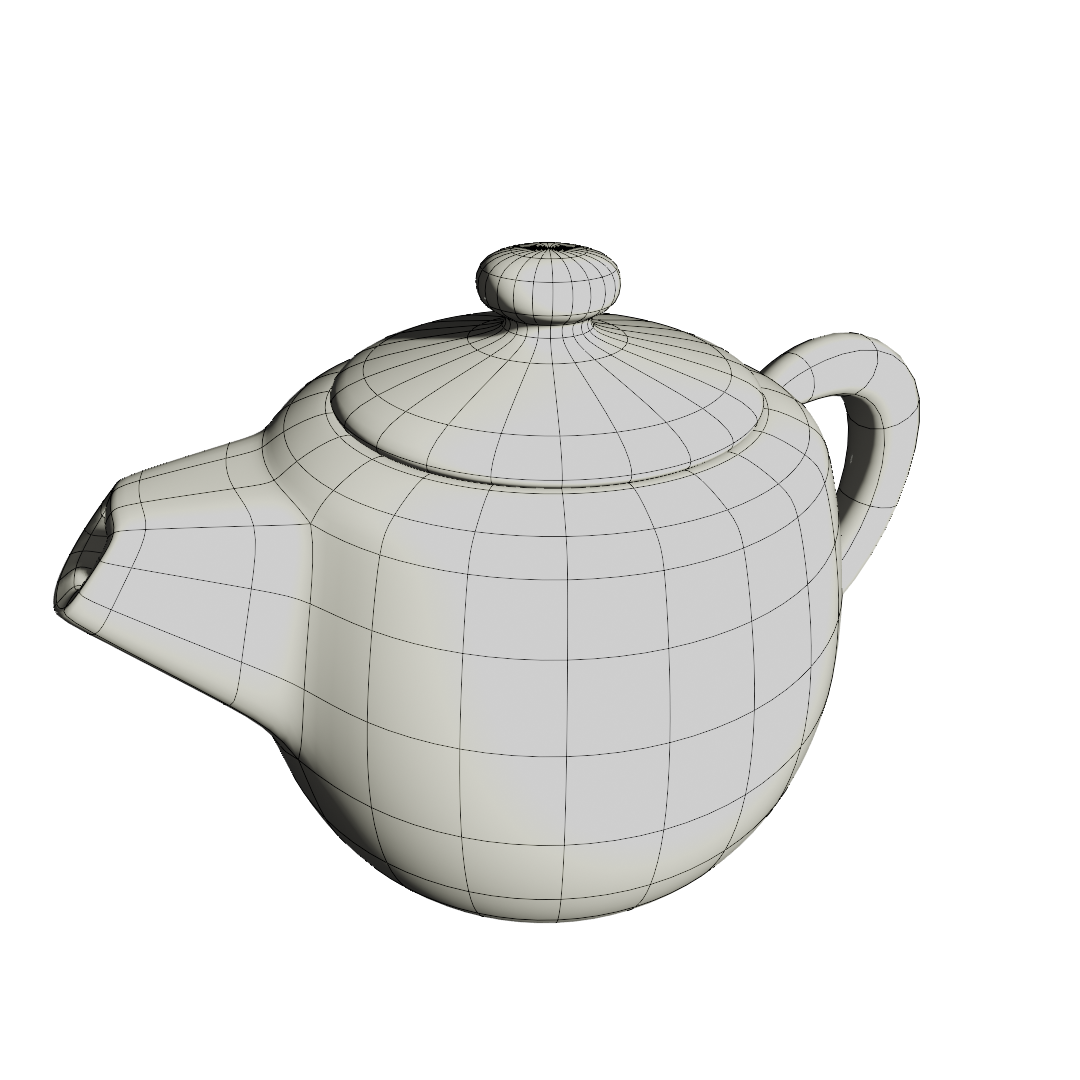
\includegraphics[scale=\myscale,scale=0.15,trim={2cm 5cm 2cm 5cm},clip]{figures/teapot}
\end{center}

\index{maillage}

%%%%%%%%%%%%%%%%%%%%%%%%%%%%%%%%%%%%%%%%%%%%%%%%%%%%%%%%%%%%%%%%%%%%%
\section{Généralités}

%--------------------------------------------------------------------
\subsection{Une définition}

Un \defi{maillage} d'une surface $E$ est un ensemble $(S,A,F)$ où :
\begin{itemize}
	\item $S$ sont des \defi{sommets}  (ici des points de l'espace),
	\item $A$ sont des \defi{arêtes} (ici des portions de courbes),
	\item $F$ sont des \defi{faces} (ici des portions de surfaces),
\end{itemize}
de telle sorte que l'union de toutes les faces soit égale à la surface $E$ de départ.

\myfigure{0.7}{
	\tikzinput{maillage-01}
}	


On impose en plus des conditions reliant sommets/arêtes/faces :
\begin{itemize}
	\item Le bord d'une arête est composé de deux sommets distincts. Tout sommet est dans le bord d'une arête. Deux arêtes ne peuvent s'intersecter qu'en un sommet.
	
	\item Le bord d'une face est formé d'arêtes distinctes. Toute arête est dans le bord d'une face. L'intersection de deux faces est une arête ou un sommet (ou rien).
\end{itemize}


Partant d'une surface originale $E$, un maillage s'obtient souvent par discrétisation de la surface, comme pour les triangulations (voir le chapitre \og{}Triangulation\fg{}).
Cependant ici les objets sont des objets de l'espace et les faces ne sont pas nécessairement des triangles. Par exemple une arête peut être une courbe de l'espace et une face n'est pas nécessairement plate.


On peut aussi considérer un maillage comme un objet combinatoire, c'est-à-dire une fois donnés les sommets $S$, une arête est juste un couple de sommets (sans description de la courbe les reliant) et une face est une liste de sommets. Il y a alors plusieurs façons de reconstruire une surface correspondant à ce maillage :

\begin{itemize}
	\item \evidence{interpolation} : on construit une courbe ou une surface qui passe par les sommets imposés,
	
	\item \evidence{approximation} : on construit une courbe ou une surface qui approche au mieux (selon certains critères) les sommets mais qui ne passe pas nécessairement par ces sommets,
	
	\item \evidence{changement de normales} : on ne modifie pas le maillage mais la manière dont l'éclairage est calculé en modifiant les vecteurs normaux à chaque face (voir le chapitre \og{}Texture\fg{}).
\end{itemize}	


\myfigure{0.5}{
	\tikzinput{maillage-02}
}	


%--------------------------------------------------------------------
\subsection{Codage}

Revenons sur la combinatoire $(S,A,F)$ d'un maillage et comment on pourrait l'encoder dans un ordinateur :
\begin{itemize}
	\item L'ensemble des sommets $S$ est une liste numérotée de points $s_i$, $i=1,\ldots,n$.
	Chaque sommet $s_i$ est déterminé par des coordonnées $(x_i,y_i,z_i) \in \Rr^3$.
	
	\emph{Données optionnelles.} À chaque sommet on associe la liste des arêtes issues de ce sommet.
	
	\item L'ensemble des arêtes $A$ est une liste numérotée d'arêtes $a_j = (i_1,i_2)$ où
	$i_1$ et $i_2$ sont les numéros des sommets $s_{i_1}$ et $s_{i_2}$ aux bords de l'arête.
	
	\emph{Données optionnelles.} À chaque arête on associe la liste des faces touchant cette arête.
	
	\item L'ensemble des faces $F$ est une liste numérotée de faces $f_k$ définies par une liste $(i_1,i_2,\ldots,i_m)$ de (numéros de) sommets.
	
	\emph{Données optionnelles.} À chaque face on associe la liste des arêtes du bord.
\end{itemize}

\medskip
Quelles sont les données du maillage dessiné ci-dessous ?

\myfigure{1.1}{
	\tikzinput{maillage-03}
}	

\begin{itemize}
	\item $S = \{s_1,\ldots,s_5\}$, avec $s_i=(x_i,y_i,z_i)$, $i=1,\ldots,5$.
	\item Les arêtes sont $A = \{a_1,\ldots,a_6\}$, avec $a_1 = \{1,2\}$ (car d'extrémités $s_1$ et $s_2$), $a_2 = \{1,3\}$, \ldots
	\item Les faces sont $F = \{f_1,f_2\}$, avec $f_1 = \{1,2,3\}$ (car déterminée par les sommets $s_1, s_2, s_3$) et  $f_2 = \{2,3,4,5\}$. 
\end{itemize}

Les données optionnelles peuvent être obtenues à partir des données initiales mais nécessitent un parcours dans ces données initiales.


%--------------------------------------------------------------------
\subsection{Quelques types d'arêtes}

Pour deux sommets $A$ et $B$ il existe de nombreuses façons de les relier.
Voyons trois méthodes.
	
\textbf{Arête rectiligne/\emph{lerp}.}\index{interpolation!lineaire@linéaire}
$$\gamma(t) = (1-t)A + tB \qquad \qquad t \in [0,1]$$
C'est l'interpolation linéaire classique (\emph{lerp}) qui dessine un arête rectiligne.
Il faut comprendre l'addition de points	comme l'addition de vecteurs 
$A= \left( \begin{smallmatrix} x_A \\ y_A \end{smallmatrix}\right)$,
$B= \left( \begin{smallmatrix} x_B \\ y_B \end{smallmatrix}\right)$ (dans le plan)
ou 
$A= \left( \begin{smallmatrix} x_A \\ y_A \\ z_A \end{smallmatrix}\right)$,
$B= \left( \begin{smallmatrix} x_B \\ y_B \\ z_B \end{smallmatrix}\right)$ (dans l'espace).

\myfigure{1.5}{
	\tikzinput{maillage-04}
}

\bigskip

\textbf{Arête circulaire/\emph{slerp}.}\index{interpolation!circulaire}
Considérons deux points $A$ et $B$ situés à une distance $R$ d'un point $O$.
Alors l'arc du cercle de centre $O$ et de rayon $R$ commençant à $A$ et finissant à $B$ est donné par :
\mybox{$\displaystyle \gamma(t) = R\frac{\sin((1-t)\omega)}{\sin \omega} A \ + \ R\frac{\sin(t\omega)}{\sin \omega} B \qquad \qquad t \in [0,1]$}
où $\omega$ est l'angle formé par les vecteurs $\vec{OA}$ et $\vec{OB}$ et est donné par la formule :
$$\vec{OA} \cdot \vec{OB} = R^2 \cos(\omega).$$

\myfigure{1.5}{
	\tikzinput{maillage-05a}
}

Par exemple en $t=\frac12$, on obtient le milieu de l'arc ; avec $t=\frac13$ et $t=\frac23$ on coupe l'arc en trois parties égales\ldots

Pour différentes valeurs du rayon on obtient des arcs plus ou moins courbés.
\myfigure{1.15}{
	\tikzinput{maillage-05b}
}

Preuve : On peut se placer dans le plan $(Oxy)$ et supposer que $A$ a pour coordonnées $(1,0)$. Notons $C$ le point de coordonnées $(0,1)$. Dans ce repère les coordonnées d'un point du cercle centré en $O(0,0)$ et de rayon $1$ sont $(\cos\theta, \sin\theta)$. 
Ainsi un point $P$ du cercle s'écrit $P = \cos(\theta) A + \sin(\theta) C$ (c'est-à-dire
$\vec{OP} =  \cos(\theta) \vec{OA} + \sin(\theta) \vec{OC}$).
En particulier $B = \cos(\omega) A + \sin(\omega) C$.

\myfigure{1.3}{
	\tikzinput{maillage-05c}
}

Ainsi $C = -\frac{\cos\omega}{\sin\omega}A + \frac{1}{\sin\omega}B$. On obtient alors :
$$P = \frac{\sin\omega\cos\theta - \sin\theta\cos\omega}{\sin\omega}A + \frac{\sin\theta}{\sin\omega}B
= \frac{\sin(\omega-\theta)}{\sin\omega}A + \frac{\sin\theta}{\sin\omega}B.$$
On pose $\theta = \omega t$ où $t \in [0,1]$ afin d'obtenir la paramétrisation de l'arc de cercle entre $A$ (en $t=0$) et $B$ (en $t=1$):
$$P 
= \frac{\sin((1-t)\omega)}{\sin\omega}A + \frac{\sin(t\omega)}{\sin\omega}B.$$
 

\bigskip

\textbf{Arête quadratique.} Ces arêtes sont données par des équations de degré $2$.
Autrement dit, ce sont des courbes de Bézier avec un seul point de contrôle.
La \defi{courbe quadratique de Bézier}\index{courbe!quadratique de Bezier@quadratique de Bézier} de $A$ à $B$ ayant le point de contrôle $C$ est la courbe paramétrée :
$$\gamma(t) = (1-t)^2 A \ + \  2t(t-1) C \ + \ t^2 B \qquad\qquad t \in [0,1]$$
La courbe démarre en $\gamma(0) = A$ et termine en $\gamma(1) = B$, elle ne passe pas par $C$. Par contre la courbe est tangente à $\vec{AC}$ en $A$ et tangente à $\vec{BC}$ en $B$. 

\myfigure{1.5}{
	\tikzinput{maillage-06}
}

Les courbes de Bézier générales seront étudiées dans le chapitre \og{}Approximation et interpolation\fg{}.

Un \defi{triangle de Bézier quadratique} est défini par $3$ sommets et $3$ points de contrôle.
\myfigure{0.6}{
	\tikzinput{maillage-07}
}



%%%%%%%%%%%%%%%%%%%%%%%%%%%%%%%%%%%%%%%%%%%%%%%%%%%%%%%%%%%%%%%%%%%%%
\section{Vecteur normal}

On rappelle que l'éclairage d'un objet est calculé à partir des vecteurs normaux à la surface (voir les chapitres \og{}Lumière\fg{} et \og{}Texture\fg{}). Changer les vecteurs normaux permet de changer l'apparence de l'objet sans toucher à la géométrie sous-jacente.

Ci-dessous de gauche à droite : le maillage d'une sphère, le rendu plat et le rendu après lissage des vecteurs normaux (sans changer le maillage).
\begin{center}
	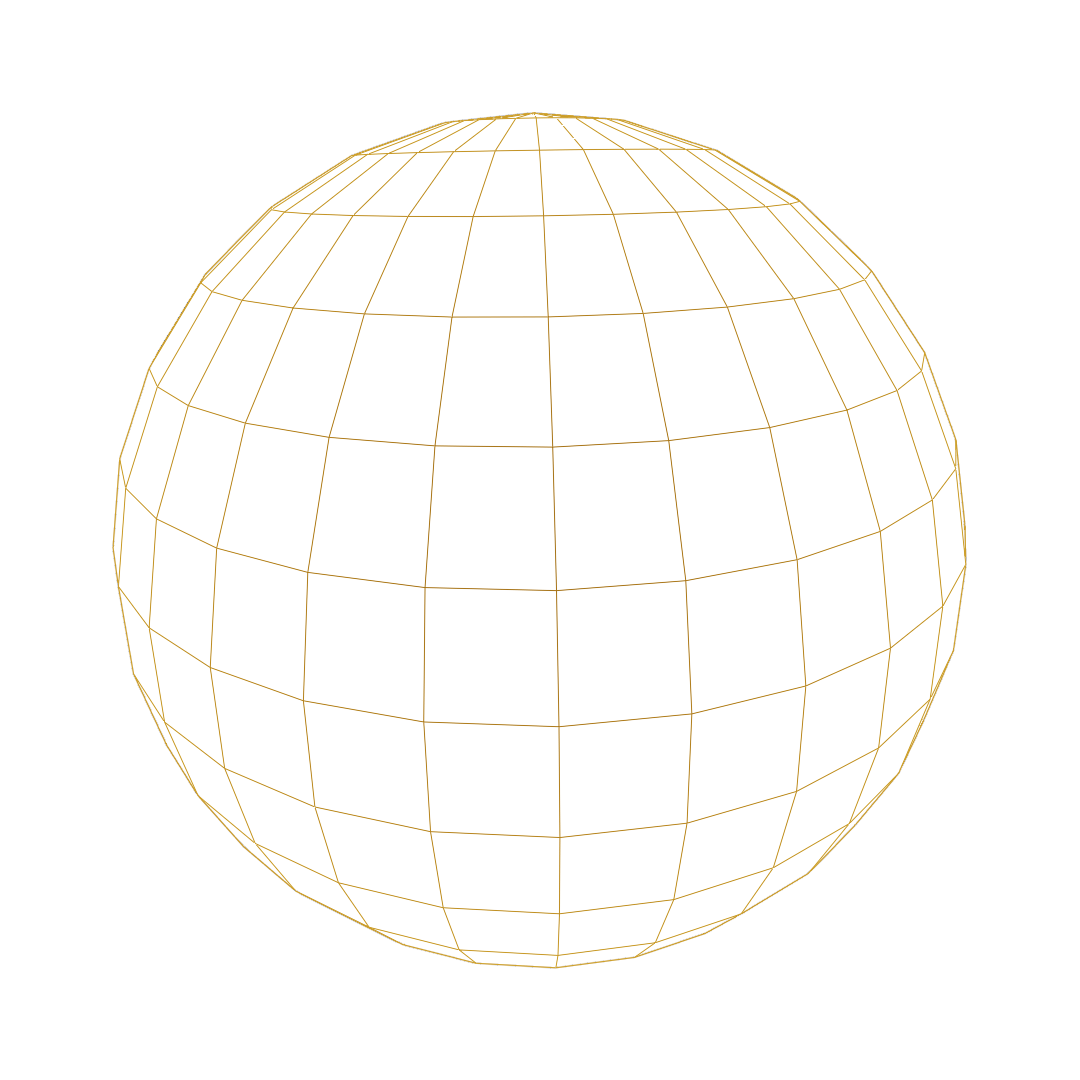
\includegraphics[scale=\myscale,scale=0.15,trim={2cm 0 2cm 0},clip,]{figures/sphere-new-00}
	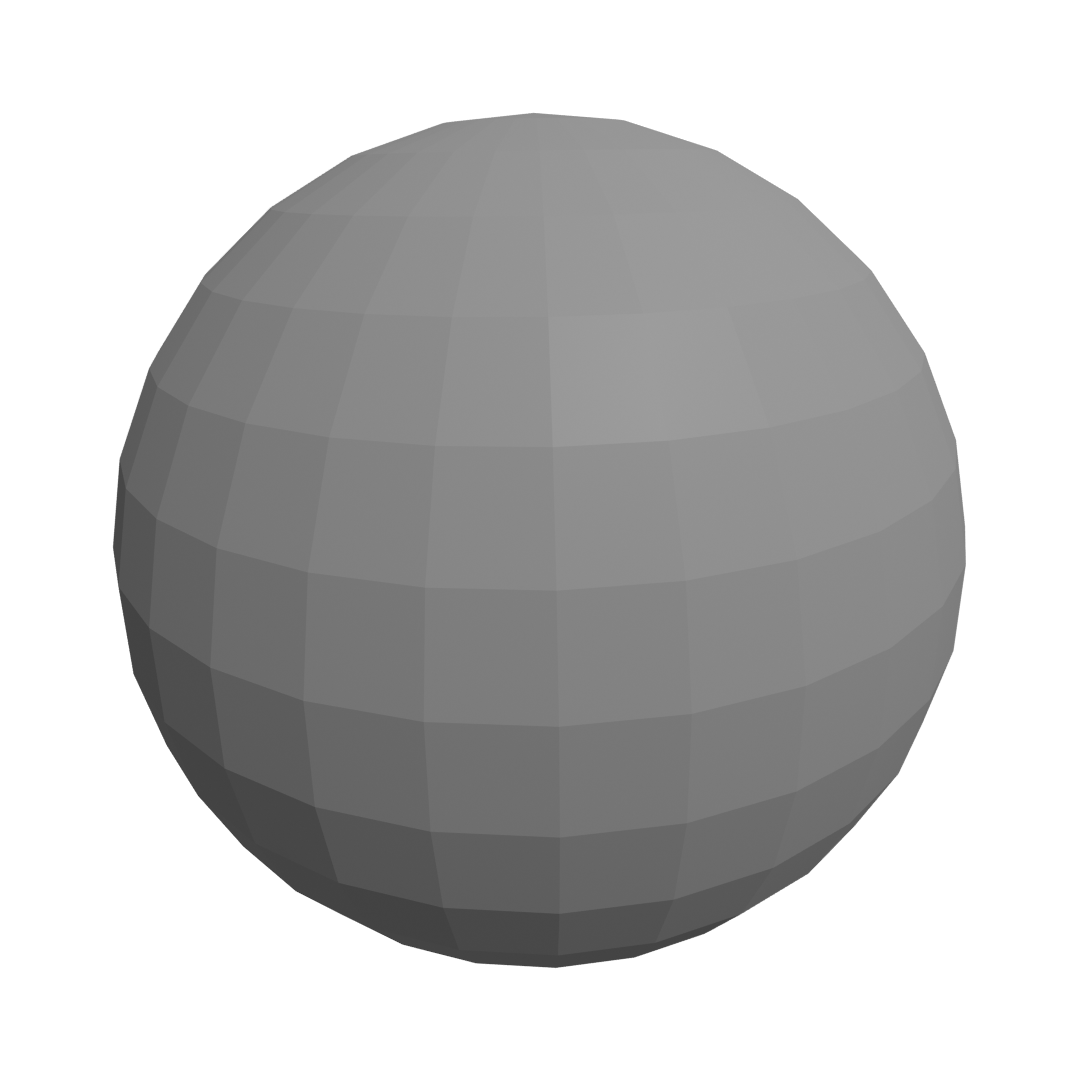
\includegraphics[scale=\myscale,scale=0.15,trim={2cm 0 2cm 0},clip,]{figures/sphere-new-02}		
	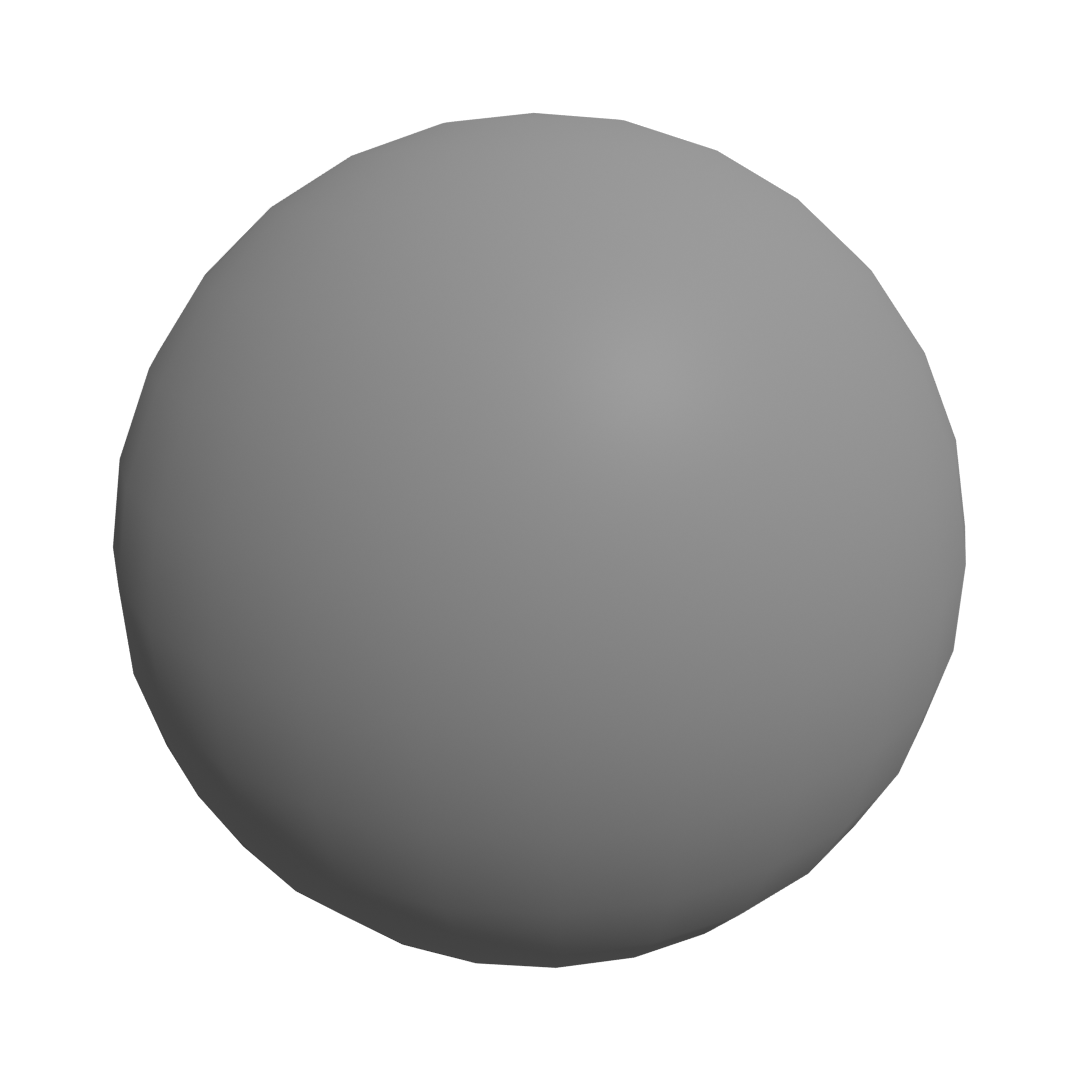
\includegraphics[scale=\myscale,scale=0.15,trim={2cm 0 2cm 0},clip,]{figures/sphere-new-03}
\end{center}

%--------------------------------------------------------------------
\subsection{Normales aux arêtes}

Nous commençons par le cas d'une arête entre deux points $A$ et $B$ dans le plan.

\textbf{Une seule normale.}
Quel que soit le point $P$ du segment $[AB]$, le vecteur normal est toujours le même (à un facteur multiplicatif près). Cela correspond à un éclairage \og{}plat\fg{}.


\myfigure{1}{
	\tikzinput{normale-01}
}




\medskip
\textbf{Une normale à chaque extrémité.}
Considérons le même segment $[AB]$ et supposons que l'on nous donne un vecteur $\vec{n_A}$ en $A$ et un vecteur $\vec{n_B}$ en $B$. On en déduit un vecteur en n'importe quel point du segment. 
Par interpolation linéaire, un point $P$ du segment s'écrit $P = (1-t)A+tB$ et en ce point on définit le vecteur :
$$\vec{n_P} = (1-t)\vec{n_A} \  + \ t\vec{n_B}$$

\myfigure{0.7}{
	\tikzinput{normale-02}
}

Il est abusif de parler de \og{}vecteurs normaux\fg{} pour les vecteurs $\vec{n_P}$ car ils ne sont en général pas orthogonaux à $\vec{AB}$. Cependant ils vont remplacer le vecteur normal lors des calculs d'éclairage et permettent de simuler une courbure entre $A$ et $B$. En fait ce sont les vrais vecteurs normaux d'une arête courbe qui sont ici ramenés sur une arête rectiligne. On renvoie de nouveau au chapitre \og{}Texture\fg{}.

\myfigure{0.6}{
	\tikzinput{normale-03}
}

\medskip
\textbf{Plusieurs arêtes.}
Comment simuler une courbe lisse à partir de plusieurs arêtes ?
(a) On détermine un (vrai) vecteur normal de chaque arête.
(b) En chaque sommet on définit un vecteur comme la moyenne de deux vecteurs normaux des arêtes adjacentes. 
(c) Par interpolation linéaire on calcule un vecteur en chaque point de l'arête.

\myfigure{0.45}{
	\tikzinput{normale-04}
}

%--------------------------------------------------------------------
\subsection{Normales à une face triangulaire}


\textbf{Une seule normale.}
Considérons un triangle $ABC$ de l'espace.
Sa normale (la vraie) est le vecteur $\vec n$ donné par $\vec{AB} \wedge \vec{AC}$ (que l'on peut rendre unitaire si on préfère).


\myfigure{1}{
	\tikzinput{normale-05}
}


\medskip
\textbf{Une normale à chaque extrémité.}
Si on impose des vecteurs $\vec{n_A}$, $\vec{n_B}$ et $\vec{n_C}$ aux sommets alors les coordonnées barycentriques remplacent l'interpolation linéaire et permettent de définir un vecteur en n'importe quel point du triangle. On renvoie au chapitre \og{}Texture\fg{} pour la définition de ces coordonnées.
Pour un point du triangle, notons $(\alpha:\beta:\gamma)$ les coordonnées barycentriques d'un point $P$ du triangle :
$$P = \alpha A + \beta B + \gamma C.$$
On définit alors le vecteur $\vec{n_P}$ par ces mêmes coefficients :
$$\vec{n_P} = \alpha\vec{n_A} + \beta \vec{n_B} + \gamma \vec{n_C}.$$

\myfigure{1}{
	\tikzinput{normale-06}\qquad\qquad
	\tikzinput{normale-07}	
}


\medskip
\textbf{Plusieurs triangles.}
Pour simuler une surface lisse à partir de plusieurs faces (triangulaires) planes.
(a) On détermine un (vrai) vecteur normal de chaque face.
(b) En chaque sommet on définit un vecteur comme la moyenne de vecteurs normaux des faces adjacentes. 
(c) Enfin on calcule un vecteur en chaque point de l'arête à l'aide des coordonnées barycentriques.


\myfigure{1}{
	\tikzinput{normale-08}	
}


%%%%%%%%%%%%%%%%%%%%%%%%%%%%%%%%%%%%%%%%%%%%%%%%%%%%%%%%%%%%%%%%%%%%%
\section{Subdivision}

Une subdivision c'est partir d'un maillage simple pour obtenir un maillage avec plus de sommets, qui est donc censé mieux représenter la surface voulue. Nous allons décrire l'algorithme de Catmull-Clark qui est une méthode de subdivision par approximation : bien sûr à la fin nous obtiendrons de nouveaux sommets, mais les sommets originaux ne sont pas conservés à leur place d'origine.

\index{algorithme!de Catmull-Clark}

%--------------------------------------------------------------------
\subsection{Subdivision combinatoire}

Commençons par décrire l'opération d'un point de vue combinatoire.
\begin{itemize}
	\item Pour chaque face on considère son centre $f$, obtenu comme isobarycentre (c'est-à-dire la moyenne) des sommets $s_1$, $s_2$,\ldots, $s_n$ définissant cette face :
	$f = \frac{s_1+s_2+\cdots + s_n}{n}$.
	
	\item Pour chaque arête de cette face on calcule son milieu $a_j$ :
	si l'arête a pour extrémité $s_{i_1}$ et $s_{i_2}$ alors $a_j= \frac{s_{i_1}+s_{i_2}}{2}$.
	
	\item On remplace la face par $n$ quadrilatères obtenus en ajoutant des arêtes reliant le centre $f$ aux milieux $a_j$ des arêtes. 
\end{itemize}

\myfigure{1}{
	\tikzinput{subdivision-01}\qquad\qquad\qquad
	\tikzinput{subdivision-02}	
}


Noter que même si la face de départ n'est pas un quadrilatère, les faces obtenues après subdivision sont toutes des quadrilatères. Dans la suite de la construction nous allons déplacer les sommets et donc, en général, les quatre sommets des quadrilatères ne seront pas situés dans un même plan.

%--------------------------------------------------------------------
\subsection{Déplacement des sommets}

Nous allons maintenant déplacer les sommets. D'une part nous allons bouger les milieux des arêtes $a_j$ que l'on vient de créer, mais en plus on va déplacer les sommets originaux $s_i$. Ces deux opérations sont indépendantes l'une de l'autre.

\textbf{Déplacement des milieux des arêtes.}

Considérons une arête d'extrémité les sommets $s_1$ et $s_2$, notons $a$ son milieu et $f_1$ et $f_2$ les centres des deux faces adjacentes. On remplace le sommet $a$ par :
$$a' = \frac{s_1+s_2+f_1+f_2}{4}$$
Ainsi $a'$ (qui servira de sommet dans la subdivision en lieu et place de $a$) est l'isobarycentre de $s_1$, $s_2$, $f_1$ et $f_2$. Comme $a= \frac{s_1+s_2}{2}$, on peut aussi dire que $a'$ est la moyenne entre : l'ancien $a$ et la moyenne des centres des faces adjacentes.

\myfigure{0.8}{
	\tikzinput{subdivision-03}	
}

 
\bigskip


\textbf{Déplacement des sommets originaux.}

\emph{Cas de $3$ faces.}
Considérons un sommet $s$ adjacent à exactement $3$ faces de centres $f_1$, $f_2$, $f_3$.
Ce sommet est alors adjacent à $3$ arêtes dont on note les milieux $a_1$, $a_2$, $a_3$ (ce sont les vrais milieux $a_j$ et pas les points déplacés $a'_j$).
On calcule la moyenne $F$ des centres des faces, la moyenne $A$ des milieux des arêtes et on effectue une moyenne pondérée pour le nouveau sommet $s'$ (qui remplace le sommet original $s$) :
$$F = \frac{f_1+f_2+f_3}{3}
 \qquad\qquad
 A = \frac{a_1+a_2+a_3}{3}
 \qquad\qquad 
 s' = \frac{F + 2A}{3}$$
 
\myfigure{0.8}{
 \tikzinput{subdivision-04}	
}
 

\emph{Cas de $n$ faces.} 
Dans le cas de $n$ faces arrivant en un sommet $s$ on remplace ce sommet $s$ par un sommet $s'$ donné par les formules suivantes :
 $$F = \frac{f_1+\cdots+f_n}{n}
\qquad\qquad
A = \frac{a_1+\cdots+a_n}{n}
\qquad\qquad
s' = \frac{F + 2A + (n-3)s}{n}$$

En termes de barycentre, $s'$ est le barycentre de sommets $f_1,\ldots,f_n$ affectés chacun d'un poids $1$ et de sommets $a_1,\ldots,a_n$ affectés chacun d'un poids $2$ et du sommet original $s$ affecté d'un poids $n-3$.


Ci-dessous de gauche à droite : (a) l'objet original est un cube (avec 6 faces), (b) on applique l'algorithme de Catmull-Clark une première fois, chaque face du cube est remplacée par $4$ quadrilatères, on obtient un objet à $24$ faces, (c) on itère le processus, (d) on itère encore. Chaque itération fournit un objet plus lisse.


\begin{center}
	\hspace*{-10mm}
	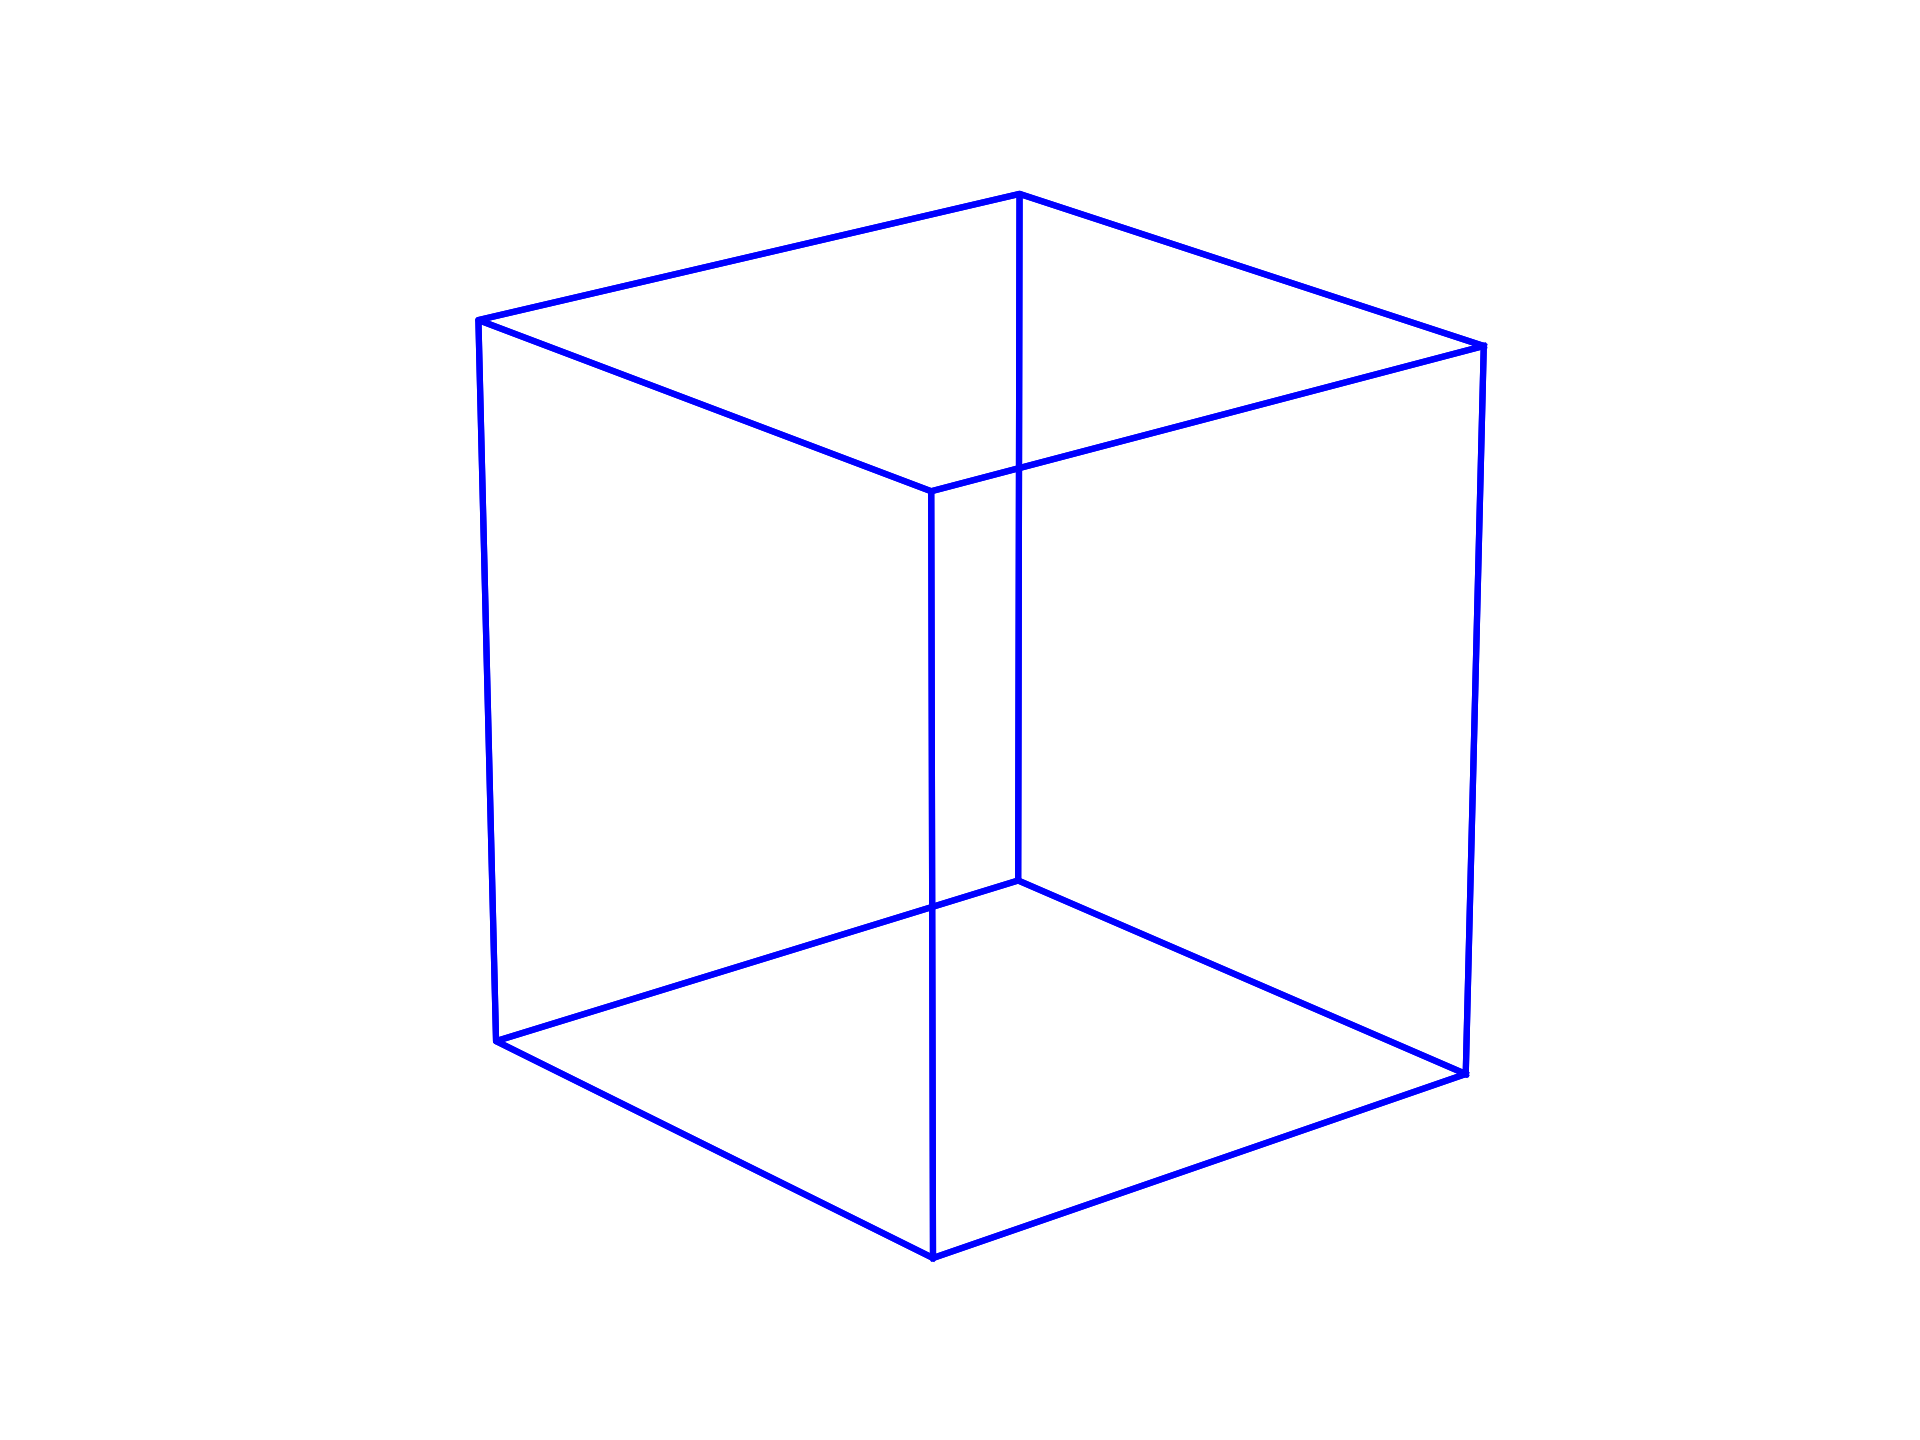
\includegraphics[scale=\myscale,scale=0.5,trim={4cm 0 3cm 0},clip,]{figures/catmull-clark-cube-0}
	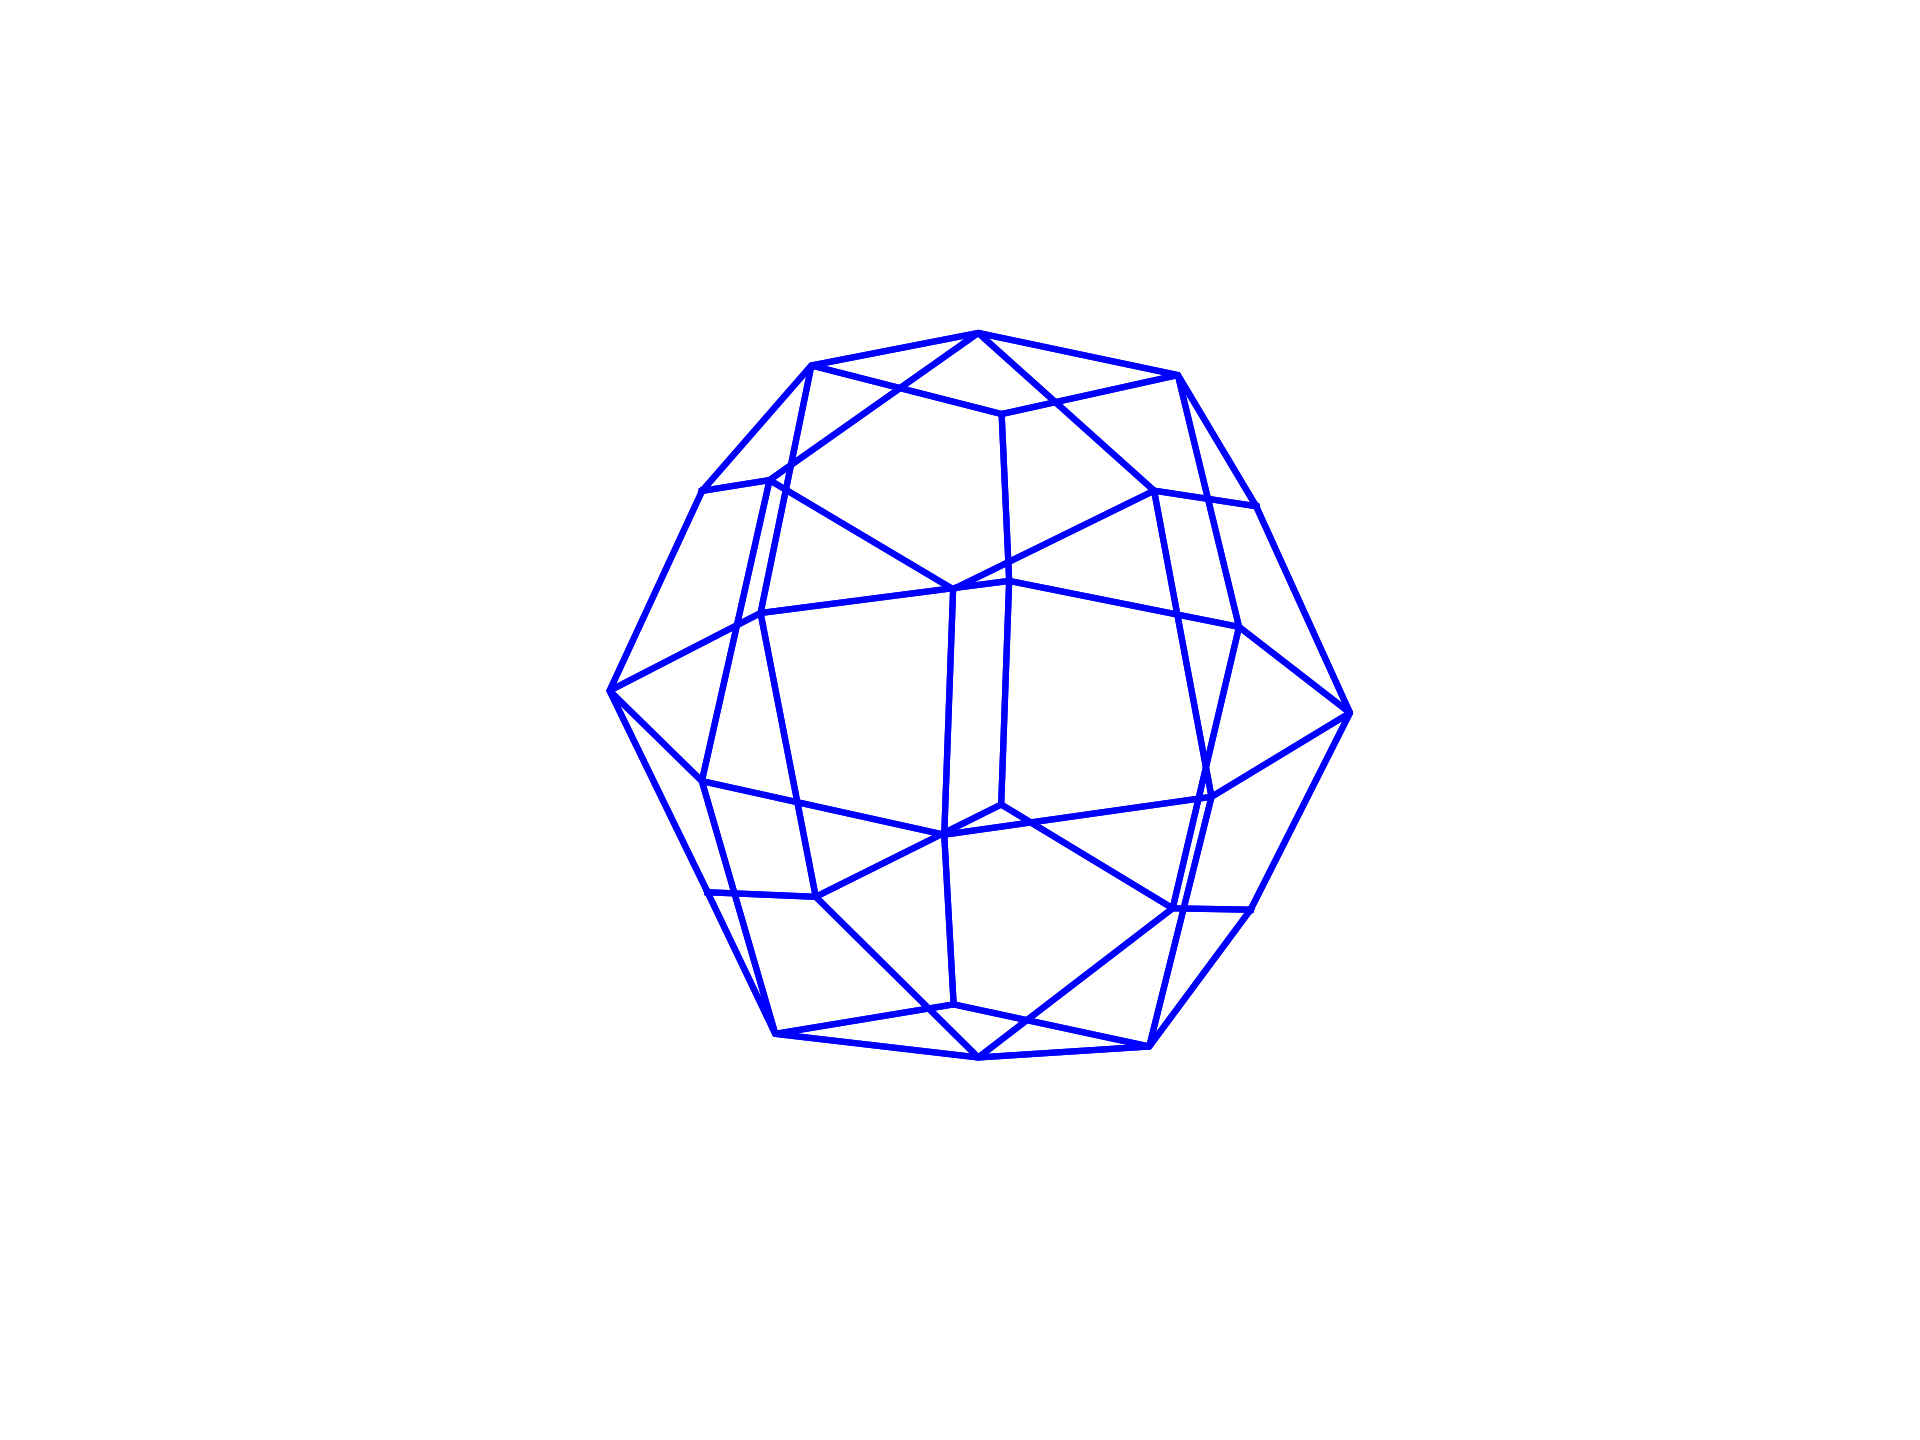
\includegraphics[scale=\myscale,scale=0.5,trim={4cm 0 4cm 0},clip,]{figures/catmull-clark-cube-1}    
	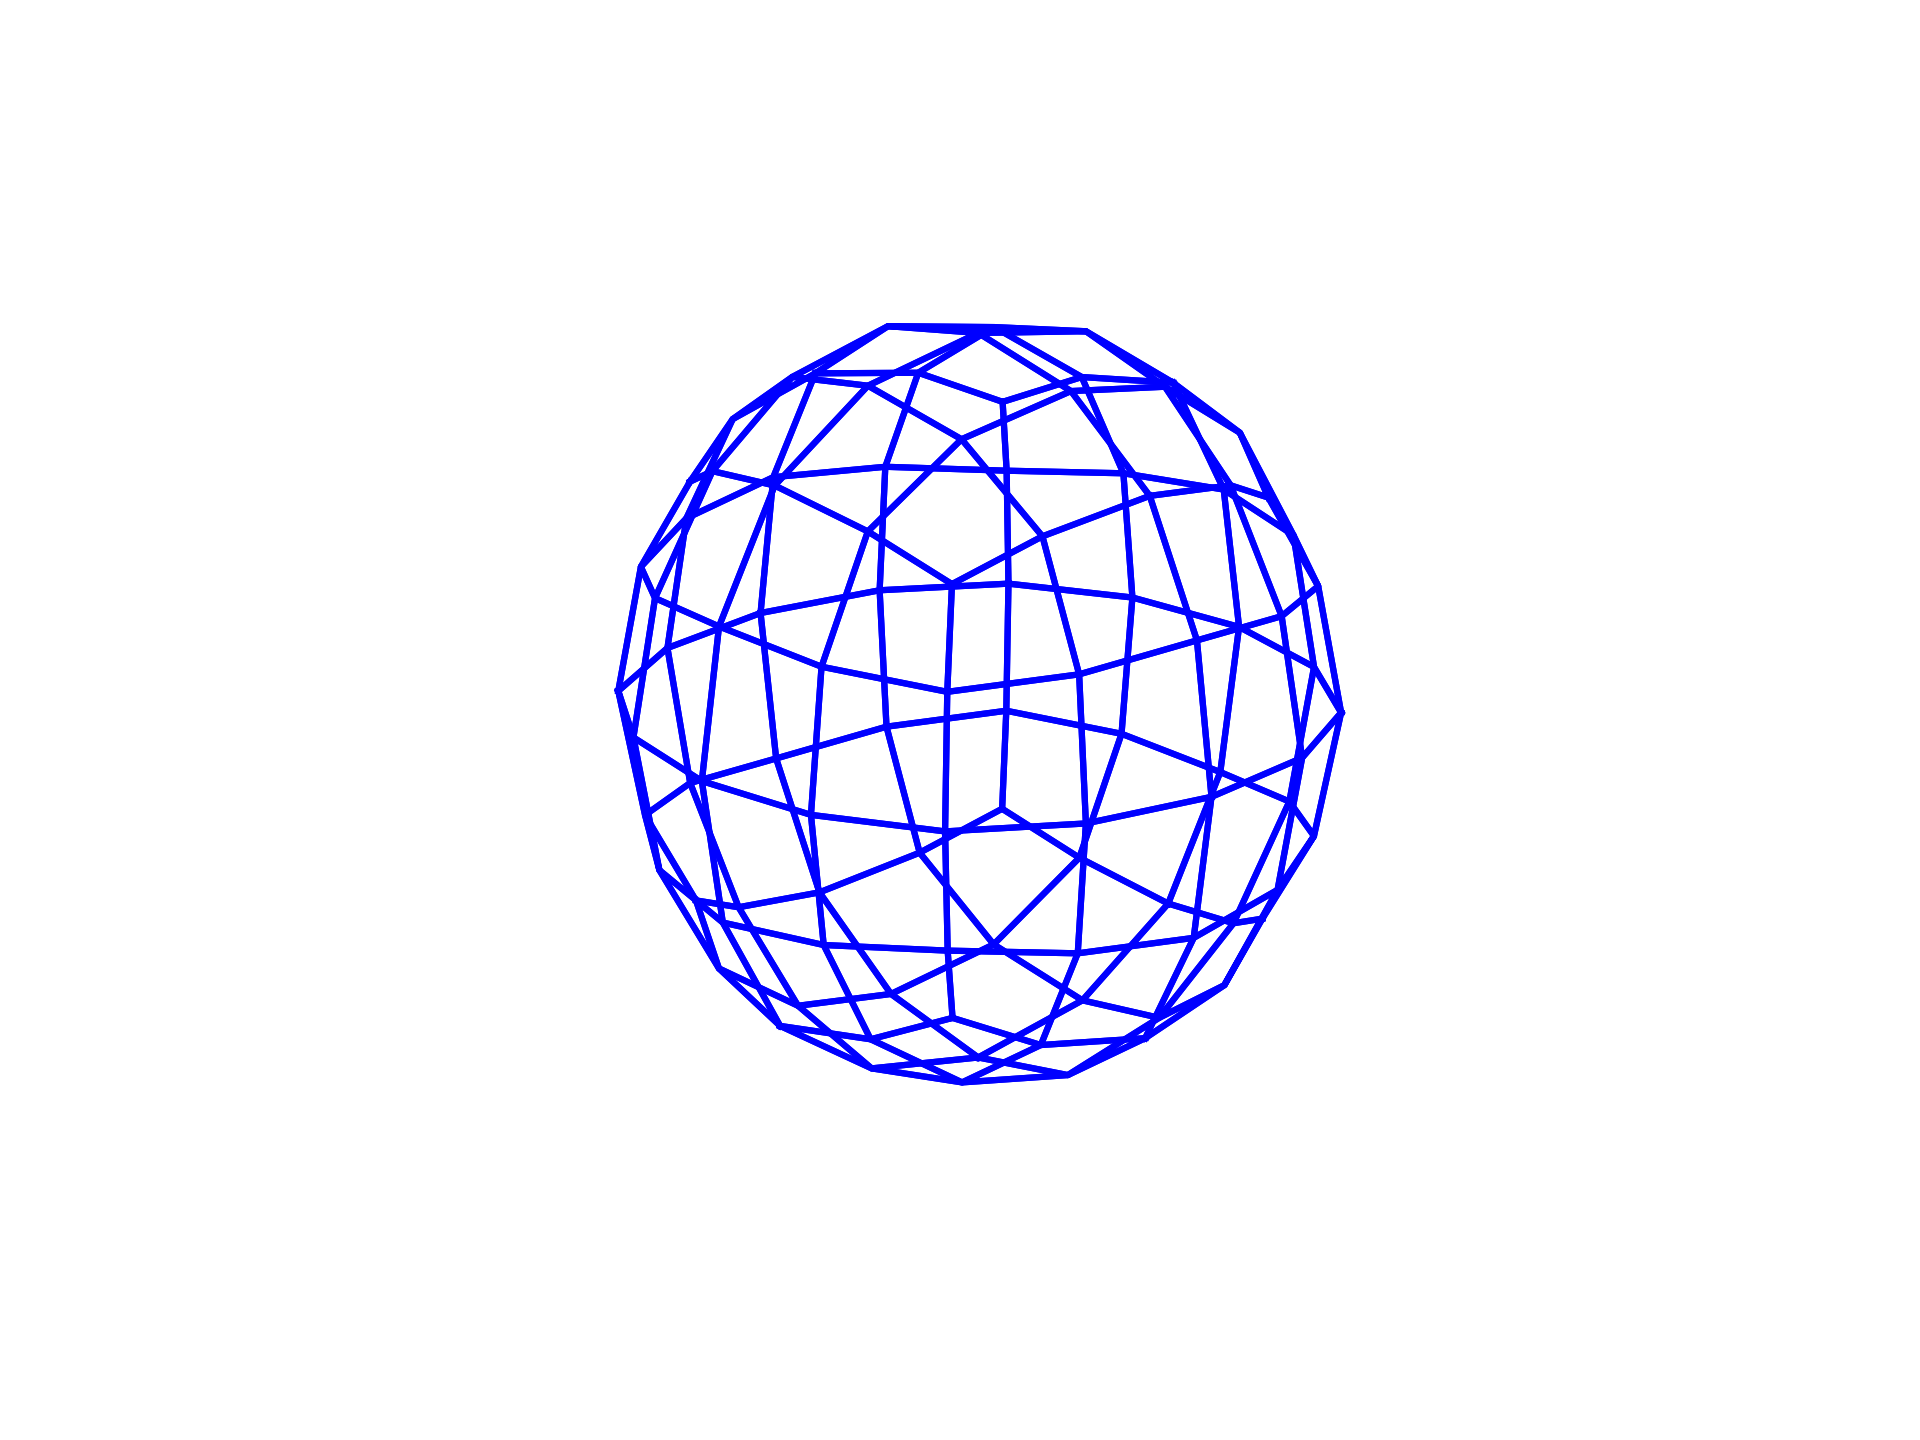
\includegraphics[scale=\myscale,scale=0.5,trim={4cm 0 4cm 0},clip,]{figures/catmull-clark-cube-2}
	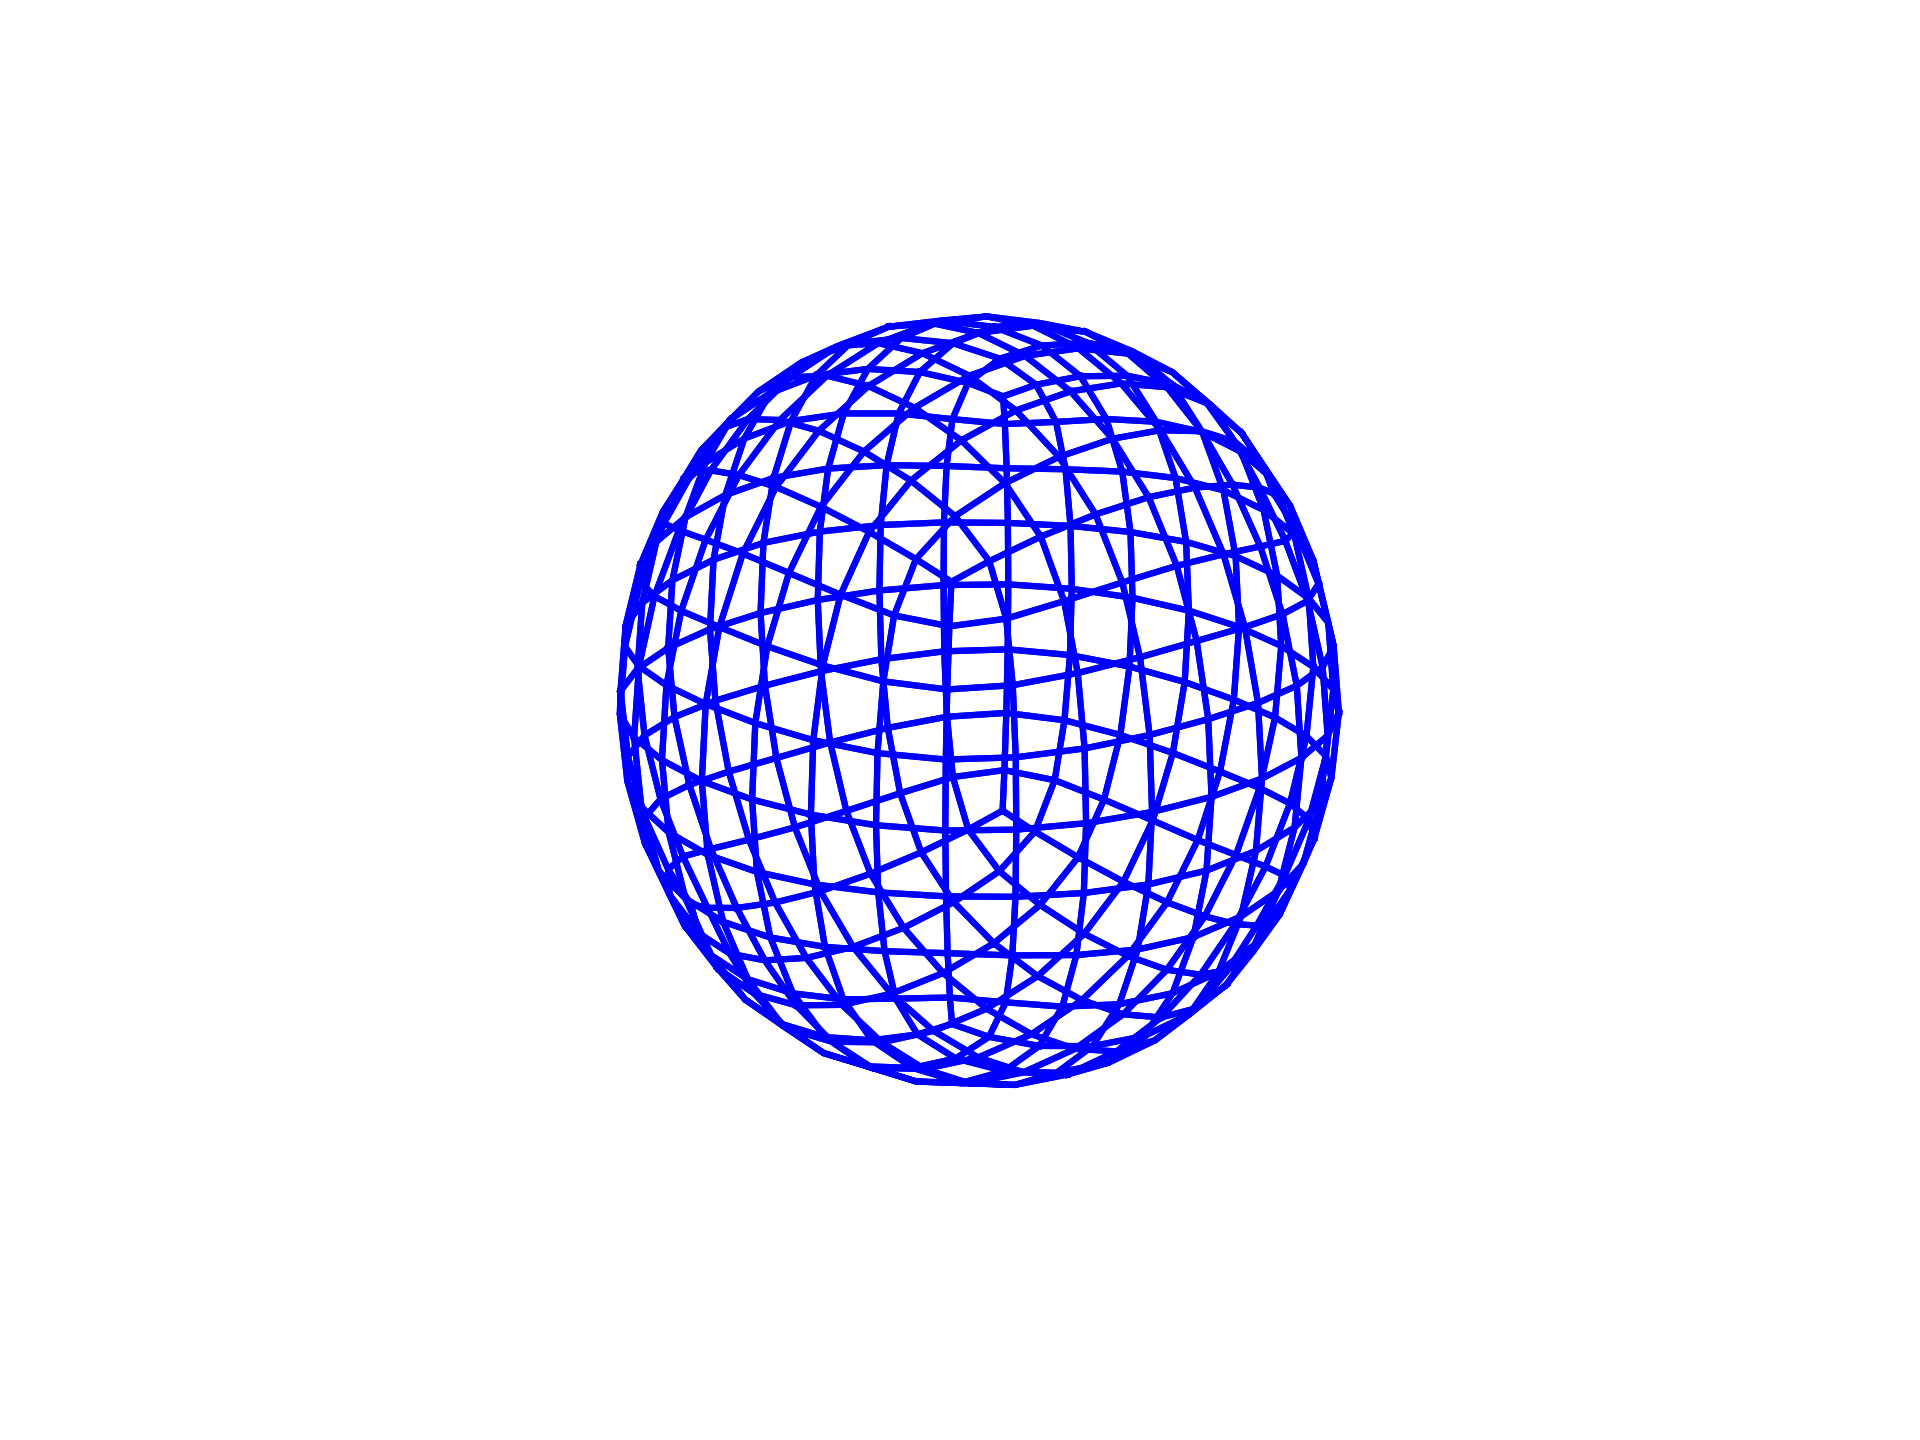
\includegraphics[scale=\myscale,scale=0.5,trim={4cm 0 4cm 0},clip,]{figures/catmull-clark-cube-3}  
	\hspace*{-20mm}  
\end{center}

De gauche à droite : (a) l'objet original, (b) une application de l'algorithme de subdivision, (c) une seconde application.
\begin{center}
 	\hspace*{-10mm}
	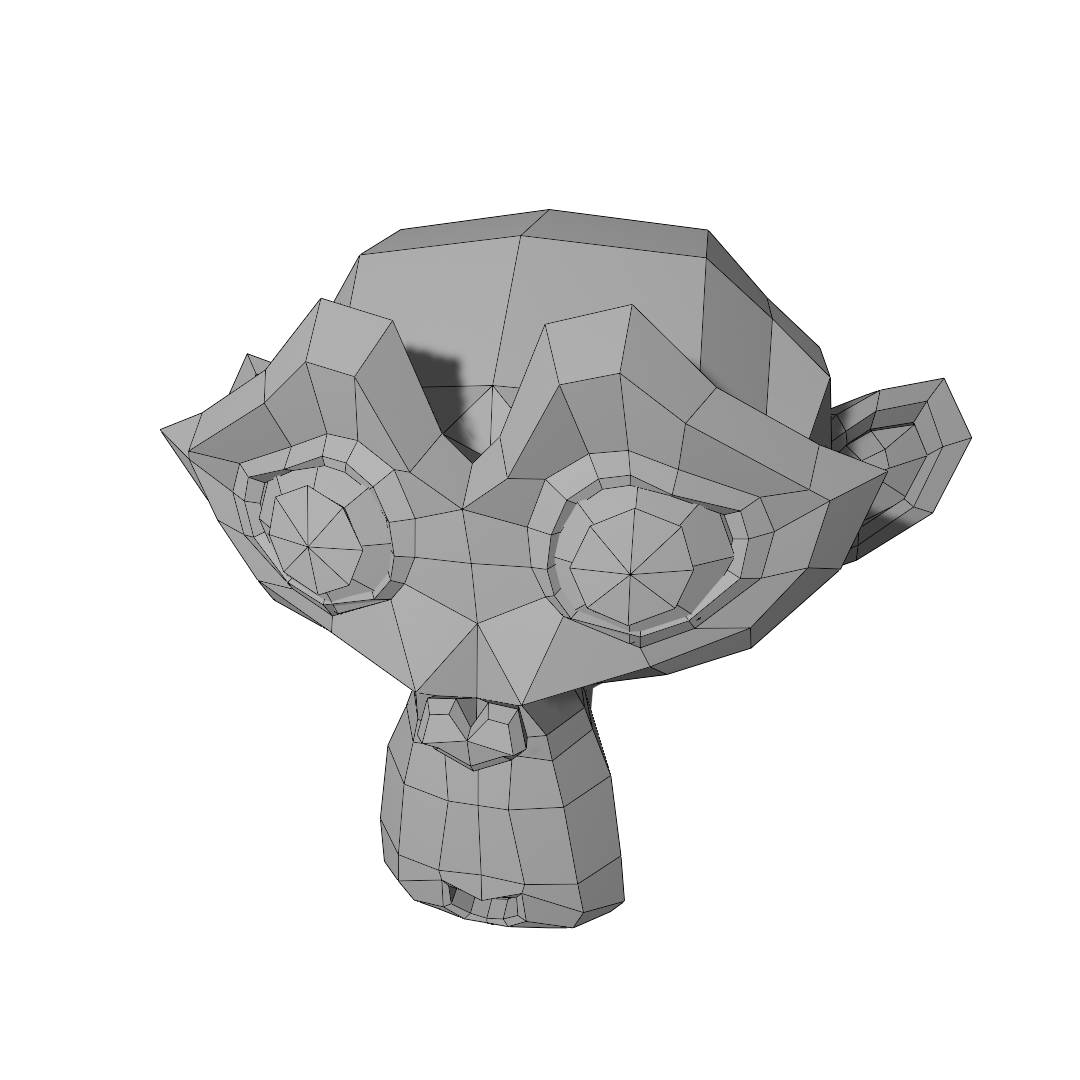
\includegraphics[scale=\myscale,scale=0.18,trim={5cm 0 4cm 0},clip,]{figures/singe-new-00}
	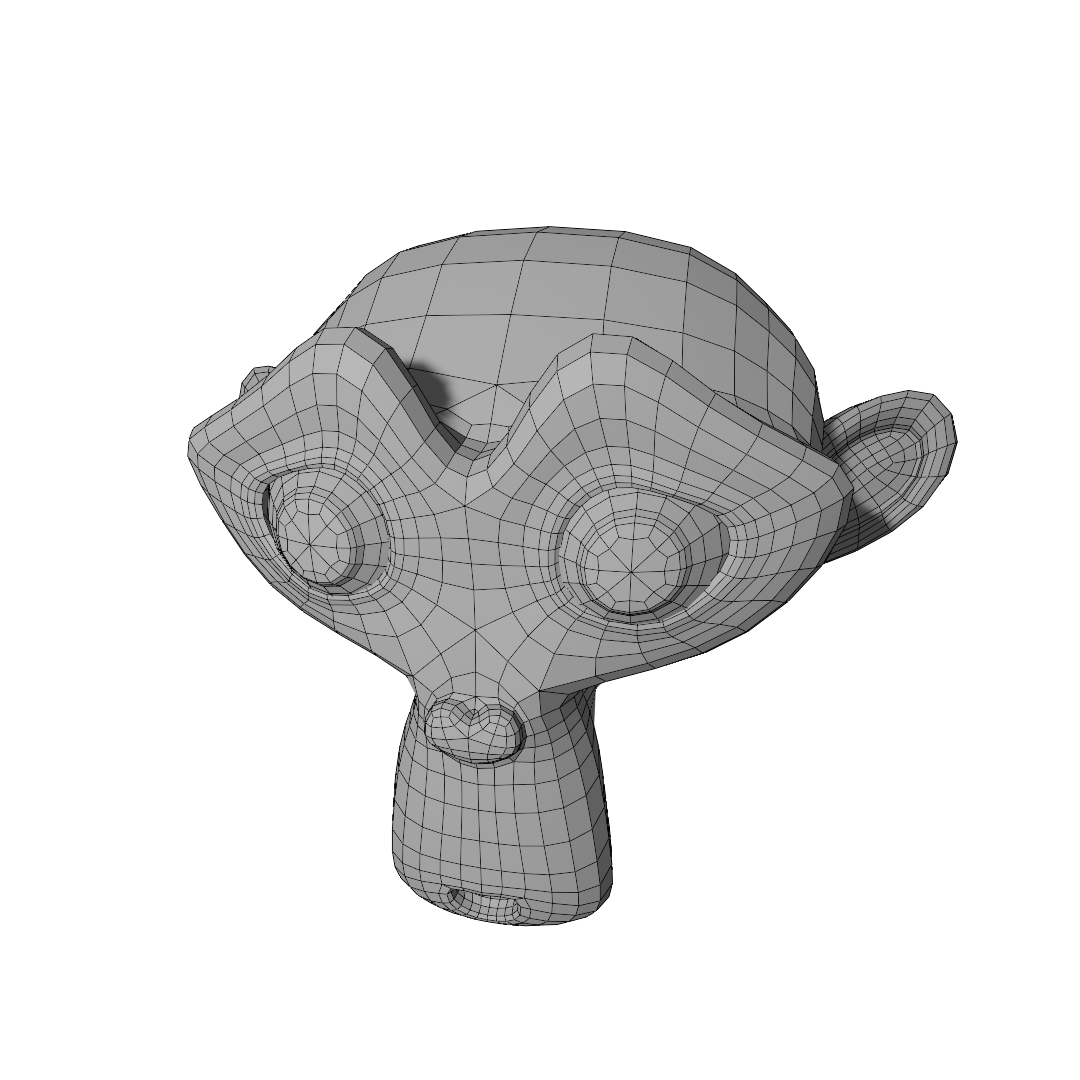
\includegraphics[scale=\myscale,scale=0.18,trim={5cm 0 4cm 0},clip,]{figures/singe-new-01}
	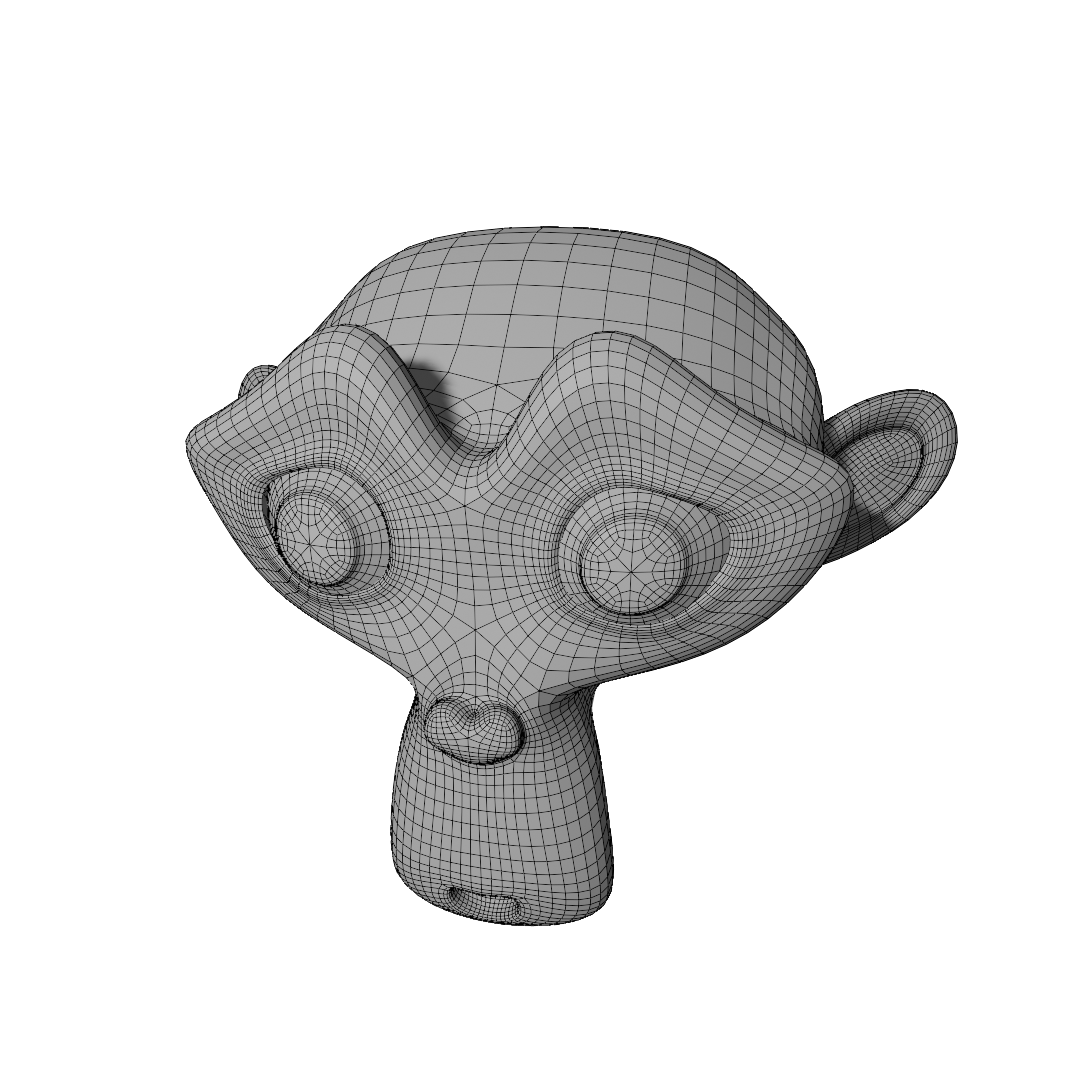
\includegraphics[scale=\myscale,scale=0.18,trim={5cm 0 4cm 0},clip,]{figures/singe-new-02}
	\hspace*{-20mm}
\end{center}


\end{document}
